%\documentclass[a4paper,11pt]{article}
\documentclass[a4paper,11pt]{article}
				
%packages will now follow
%Packages here is just for aestestics%%
\usepackage{lmodern}
\usepackage[T1]{fontenc}
%%%%%%%%%%
\usepackage[hmargin={25mm,25mm},vmargin={25mm,25mm}]{geometry}
\usepackage{amsmath,amsfonts,amsthm} %math package
\usepackage{breqn}  %math package
\numberwithin{equation}{section}
\usepackage{float}
\usepackage{graphicx}
\usepackage[outdir=./Graphs/]{epstopdf}
%%%%%%%%%%%%%%%%
\usepackage{hyperref}
\usepackage{bigints}
\usepackage{enumerate}
\usepackage{parskip}
\usepackage{wrapfig}
\usepackage{lipsum}
\usepackage{lscape}
\usepackage{threeparttable}
\usepackage{longtable}
\usepackage{multirow}
\usepackage{caption,booktabs,array}
\usepackage{url}
\usepackage{xspace}
\usepackage{tabto}
\usepackage{pdflscape}
\usepackage{chngcntr}
\usepackage[bottom]{footmisc}
%\counterwithout{footnote}{chapter}
\usepackage[nottoc]{tocbibind}
\usepackage{setspace} 
%\onehalfspacing
\doublespacing
\usepackage{xcolor}

%\usepackage{babel}

\setlength{\extrarowheight}{3pt}

\newcommand{\rowgroup}[1]{\hspace{-1em}#1}
\newcommand\cites[1]{\citeauthor{#1}'s\ (\citeyear{#1})}
\newcommand\citesall[1]{\citeauthor*{#1}'s\ (\citeyear{#1})}
\newcolumntype{P}[1]{>{\centering\arraybackslash}p{#1}}

\usepackage{tocloft}
\renewcommand{\cftfigfont}{Figure }
\renewcommand{\cfttabfont}{Table }
%\renewcommand{\bibname}{List of References}

\usepackage{fancyhdr}
\pagestyle{fancy}

\fancyhead[C]{}
\fancyhead[R]{}
\fancyhead[L]{}

\fancyfoot[C]{\thepage}
\fancyfoot[R]{}
\fancyfoot[L]{}

\renewcommand{\headrulewidth}{0pt}
\renewcommand{\footrulewidth}{0pt}

\usepackage{array}
\newcolumntype{x}[1]{>{\centering\arraybackslash\hspace{0pt}}p{#1}}

\usepackage{natbib}

\setlength{\parindent}{0cm}
\setlength{\parskip}{1.3ex plus 0.5ex minus 0.3ex}

\graphicspath{{Graphs/}}
\usepackage[font=small]{caption}

\title{\textsc{A medium-sized, open-economy, fiscal DSGE model of South Africa}\footnote{This paper represents and edited version of a chapter contained in the author's original PhD dissertation, entitled \textit{Essays on fiscal policy in South Africa}, completed at the University of Stellenbosch. Original copyright belongs to the University of Stellenbosch.}}
\author{Johannes Hermanus Kemp}


%-----------------------------------------------------------------------------------------------------------------------------

\begin{document}
	
%-----------------------------------------------------------------------------------------------------------------------------

\maketitle
	\thispagestyle{empty}
	\noindent\rule{16.5cm}{0.4pt}
	
	\begin{abstract}
		  \noindent Much of the research on fiscal multipliers has used reduced-form modelling approaches. While these models have been extended to include richer controls and innovative identification approaches, a question that often arises is whether shocks identified in these models capture the true structural shocks. An alternative and more theoretical way to identify shocks to government spending and taxes is through DSGE models. To that end, this paper estimates an open-economy DSGE model in the New Keynesian tradition, but with a more detailed fiscal block, to improve our understating of the impact of fiscal policy shocks on macroeconomic outcomes in the South African context. Policy simulations indicate that government spending and investment multipliers are generally positive, albeit smaller than one. Secondly, it is found that taxes are highly distortionary, with large negative multipliers for private consumption and investment. In contrast, the impact of tax shocks on output is ambiguous and depends on assumptions regarding the functional form of the different fiscal rules. Finally, simulations suggest that government consumption spending and, to a lesser extent, labour and consumption taxes are the most effective instruments for stabilising debt after a fiscal shock. 
	\end{abstract}
	
	\noindent\rule{16.5cm}{0.4pt}
	
	%\tableofcontents
	
%\vfill

\textbf{JEL Classification:} C32, E32, E62, H62, H63
	
\textbf{Keywords:} DSGE model; fiscal policy; fiscal multiplier; Bayesian inference 
	
\newpage
\pagenumbering{arabic}


\section{Introduction}
	
	Much of the research on fiscal multipliers has used reduced-form modelling approaches. While these models have been extended to include richer controls and innovative identification approaches in an effort to refine the analysis, a question that often arises is whether shocks identified in these reduced-form models, more often than not with minimal theoretical restrictions, capture the \textit{true} structural shocks. 
	
	An alternative, more theoretically way to identify shocks to government spending and taxes is through estimated dynamic stochastic general equilibrium (DSGE) models. Given their theoretical consistency and inherently forward-looking nature, DSGE models present a useful tool for policy analysis, and fiscal policy analysis in particular. The rational expectations paradigm embedded in the DSGE framework imply that agents' beliefs about which fiscal instruments are used to finance public debt play a crucial role in the determination of the equilibrium as well as the dynamic response of endogenous variables, including output. 
	
	In light of these considerations, an open-economy DSGE model in the New Keynesian tradition, but with a more detailed fiscal block as in \cite{coenen2013}, is estimated in an attempt to improve our understating of the size (and direction) of the impact of fiscal policy shocks on macroeconomic outcomes in the South African context. Apart from the now standard set of nominal rigidities, the model contains several features that make it suitable for fiscal policy analysis, namely non-Ricardian (or rule-of-thumb) consumers, utility-enhancing government spending, and distortionary taxes.
	
	Despite the international interest in estimating the impact of fiscal shocks on macroeconomic outcomes, very little work has been done in the South African context. A notable exception is \cite{jooste} who investigated the impact of fiscal policy shocks using three models: a medium-scale, closed-economy DSGE model, a (open-economy) structural vector error correction model (SVECM), and a time varying parameter vector autoregression (TVP-VAR). The use of these non-standard models allows the authors to answer some of the important questions raised in the field pertaining to the weaknesses of standard VARs (mentioned above). The authors found that increases in government expenditure have a positive effect on GDP in the short run (albeit less than unity in some instances), but that the impact becomes negligible in the long run. Similar results hold for changes to tax policy.
	
	Policy simulations based on the estimated model indicate that government spending and investment multipliers are generally positive, albeit smaller than one. Secondly, it is found that taxes are highly distortionary, with large negative multipliers for private consumption and investment. In contrast, the impact of tax shocks on output is ambiguous and depends on assumptions regarding the functional form of the different fiscal rules. Finally, an investigation into debt dynamics suggests that government consumption spending and, to a lesser extent, labour and consumption taxes are the most effective instruments for stabilising debt after a fiscal shock. 
	
	
	\section{Literature review} \label{lit_rev}
	
	As mentioned before, while the international literature is filled with studies into the effects of fiscal policy on macroeconomic outcomes, no consensus has been reached on the size (or sign) of government spending multipliers. 
	
	In order to reconcile the theoretical predictions with results from the empirical literature, recent studies in the DSGE literature has recognised the heterogeneity in consumer behaviour apparent in the data and moved away from the restrictive assumption of the representative, infinitely-lived, rational agent. \cite{mankiw} argued that models that contain both Ricardian and non-Ricardian agents (that do not have access to financial markets and, as such, cannot save or borrow to augment consumption expenditure) is better suited for fiscal policy analysis. The seminal contribution by \cite{gali} embedded rule-of-thumb (or non-Ricardian) agents in a standard monetary New Keynesian model. They found that the presence of these rule-of-thumb consumers, together with sticky prices and deficit financing, produces sizeable positive fiscal multipliers in the model economy.
	
	Subsequent literature embedded this idea of rule-of-thumb consumers in the class of models of \cite{smets2005,smets2007} and \cite{christiano2005}. These models incorporate many of the features that have been shown to be useful in accounting for different aspects of the variation in macroeconomic aggregates, such as sticky prices, sticky wages, investment adjustment costs, habit persistence, etc. These richer models were shown to match the data reasonably well and could be used to generate estimates of the quantitative importance of rule-of-thumb consumers. Seminal examples of efforts in that direction can be found in \cite{coenen2005}, \cite{erceg2006}, \cite{rabanal2006} and \cite{forni2009}. 
	
	%In contrast to \cite{gali}, \cite{coenen2005} found that little evidence that government spending shocks crowd in consumption, mainly because the estimated share of rule-of-thumb consumers is relatively low for the Eurozone. In contrast, \cite{erceg2006} found large, positive short-run fiscal multipliers associated with temporary increases in government spending. Similarly, \cite{rabanal2006} found that private consumption increases after a government spending shock when non-separability in consumption-hours and/or non-Ricardian behaviour are introduced in the model.  
	
	Most of the early literature focused on lump-sum taxes and aggregate government spending. \cite{forni2009}, among others, extended the framework of \cite{christiano2005} and \cite{gali} by including a detailed fiscal block. On the revenue side, the authors considered different distortionary tax rates, embedded in simple policy rules. On the expenditure side, they considered government consumption excluding compensation for public employees (or government purchases of goods and services) and modelled public employment separately in order to gauge the differential impact of the different types of spending. They found that shocks to government purchases of goods and services and public sector compensation have small and temporary effects on macroeconomic aggregates, while shocks to transfers have a slightly larger and more permanent effect. The effects are more significant on the revenue side, with cuts in labour and consumption taxes inducing sizeable consumption and output responses, while reductions in capital taxes have a positive effect on private investment and total output in the medium run. 
	
	This highlights the importance of studying the underlying mix of government spending and tax decisions rather than just aggregate quantities (see, for example, \cite{mountford}, \cite{carvalho2011}, and \cite{coenen2012}).
	
	%\cite{mountford} found substantial multipliers for the US that are comparable to those of \cite{blanchard2002}, but emphasized that tax cuts are more effective in stimulating demand than increases in government spending as the private consumption response to government spending increases is insignificant. In a similar vein, \cite{coenen2012} used a version of the European Central Bank's New Area-Wide Model extended to include a detailed specification of the fiscal sector and found that discretionary fiscal measures implemented during the GFC increased annualized quarterly real GDP growth by up to 1.6 percentage points. However, the authors noted that a detailed modelling of the fiscal sector and the incorporation of several fiscal time series were pivotal for the result. \cite{carvalho2011} further distinguished between private and public capital accumulation and provides a mechanism through which public capital augments factor productivity in the private sector. This provides an additional avenue through which fiscal policy decisions can impact on real macroeconomic outcomes. 
	
	%An alternative approach that seeks to mimic the positive wage and consumption responses often found in the empirical literature entails the introduction of a different habit formation process on the part of consumers. \cite{ravn2010} developed a model of deep habits, which manages to produce positive consumption effects following a government spending impulse.\footnote{Deep habits imply that households form habits over sub-categories of consumption goods, such as cars and clothing, as opposed to aggregate consumption.}  \cite{christoffel2011} introduced a specific form of habit formation in the composite of consumption and leisure (as in \citealp{jaccard2010}) in order to study their model's ability to generate a realistic bond premium, but at the same time find significant fiscal multipliers. 
	
	A further aspect of the policy response to the GFC that received little attention initially but has gained prominence recently is the fact that monetary and fiscal policy reacted \textit{jointly} in an effort to stimulate demand. This interaction has important implications for the size of the fiscal multiplier. 
	
	Furthermore, the interaction between monetary and fiscal policy is particularly important in recessions and expansion phases of the business cycle. In fact, a common finding in the literature is that fiscal policy appears to be more effective during periods of economic downturn than during expansions (see \citealp{auerbach}; \citealp{baum2012}; \citealp{owyang2013}; \citealp{auerbach2014}; \citealp{canzoneri2015}, among others). For South Africa, using a time varying parameter vector autoregression (TVP-VAR), \cite{jooste} found fiscal multipliers that differ across time and between expansions and recessions. 
	
	{\color{red}{Several extensions have sought to enrich the basic model specifications in order to more closely resemble actual economies. One such extension is the inclusion of a mechanism for fiscal foresight on the model economy. According to \cite{ramey2011b} and \cite{leeper2012}, models that do not explicitly account for foresight is misspecified and biased responses. As shown in \cite{jooste2017}, fiscal foresight eliminates the results of \cite{gali} in that a large share of rule-of-thumb consumers is not enough to generate positive co-movement between government spending and consumption. However, under certain calibrations, the inclusion of sticky wages still generates positive consumption responses and produces sizeable output multipliers.}}
	
	The greater proportion of the literature on fiscal multipliers focus on closed economies in the vein of \cite{gali}. While some studies have investigated the impact of fiscal policy decisions within the context of an open economy (see \citealp{erceg2006}; \citealp{cavallo2007}; \citealp{ratto2007}; \citealp{levine2009}; \citealp{horvath2014}; \citealp{petros2019} for examples), this is much less prevalent. This aspect is particularly important in the context of the South Africa economy and given the assertion in the literature that fiscal multipliers are generally smaller in an open economy setting.
	
	Finally, despite the international interest in estimating the impact of fiscal shocks on macroeconomic outcomes, very little work has been done in the South African context. A notable exception is \cite{jooste} who investigated the impact of fiscal policy shocks using three models: a medium-scale, closed-economy DSGE model, a (open-economy) structural vector error correction model (SVECM), and a time varying parameter vector autoregression (TVP-VAR). The use of these non-standard models allows the authors to answer some of the important questions raised in the field pertaining to the weaknesses of standard VARs (mentioned above). The authors found that increases in government expenditure have a positive effect on GDP in the short run (albeit less than unity in some instances), but that the impact becomes negligible in the long run. Similar results hold for changes to tax policy.
	
	This paper adds to the burgeoning fiscal DSGE literature by extending the baseline closed-economy model to an open economy setting, while at the same time including a more detailed fiscal sector and estimating key parameters. 
	
	\section{The Model} \label{model_dsge}

	% % % % % % % % % % % % % % % % % % % % % % % % % HOUSEHOLDS % % % % % % % % % % % % % % % % % % % % % % % % % % % % % % % % % %
	
	The small open economy model structure closely follows that of \cite{adolfson2007} and \cite{christoffel2008}, while incorporating a more active role for fiscal policy along the lines of \cite{coenen2013}.\footnote{See \cite{steinbach2014} for an application of the \cite{adolfson2007} model to South Africa.}
	
	The basic open economy structure is relatively standard: Households consume both domestic and imported consumer goods, while optimizing agents can invest in domestic and foreign bonds. The optimizing households rent capital to firms and decide how much to invest each period, with changes to the rate of investment, as well as changes to the rate of capital utilisation, subject to adjustment costs. Each household supplies a differentiated labour service to firms, allowing them to set their wage in a \cite{calvo1983} manner. 
	
	The model contains three types of firms: domestic producers, importers and exporters. Domestic firms employ labour and capital in production. A differentiated good is produced by each type of firm. Prices are set following \cites{calvo1983} model, but with a variation that allows for the indexation to past inflation (following \cite{rabanal2006}).
	
	Finally, monetary policy follows a standard Taylor-type rule, while	the foreign economy is assumed to be exogenous.
	
	This basic specification is extended along the lines of \cite{coenen2013} to include a more active role for fiscal policy. The specification of the fiscal sector balances the need for a high degree of detail, which is essential for analysing the quantitative effects of fiscal policy innovations, and tractability, which allows for the identification of the relevant transmission mechanisms. Specifically, the model includes (i) non-Ricardian (or rule-of-thumb) consumers to facilitate a direct transmission mechanism for government transfers, (ii) government consumption that enters the households' utility function in a non-separable way, (iii) public capital which can either be a complement or substitute for private capital, (iv) time-varying distortionary taxes, and (v) a set of fiscal rules governing the endogenous response of fiscal variables.
	
	\subsection{Fiscal Authority} \label{fiscal}
	
	The fiscal authority purchases the public consumption good, $G_t$, invests in public capital, $I_{G,t}$, issues bonds to refinance its debt, $B_t$, makes transfer payments, $TR_t$, and levies different types of taxes. The fiscal authority's period-by-period budget constraint has the following form:
	
	\begin{multline} \label{fisc_budget}
	P_{G,t}G_t +P_{I_G,t}I_{G,t}+B_t+TR_t = \\\tau_t^cP_{C,t}C_t +\tau_t^wW_tN_t +\tau_t^k\left(R_{K,t}u_t-\left(\Gamma_u(u_t)+\delta\right)P_{I,t}\right)K_t+\frac{B_{t+1}}{R_t}
	\end{multline}
	
	where $P_{G,t}$ and $P_{I_G,t}$ are the prices of the public consumption good and the public investment good respectively which, under the assumption of full home bias, is just equal to the domestic price level, $P_{H,t}$. \footnote{Note that the aggregate quantity of a household specific variable, $X_{h,t}$ is given by $X_t=\int_{0}^{1}X_{h,t}dh=(1-\omega)X_{i,t}+\omega X_{j,t}$.}
	
%	Following \cite{leeper2010}, \cite{coenen2012}, \cite{born2013}, and \cite{leeper2017}, among others, fiscal policy follows rules that embed two important features. First, there may be some automatic stabilizer component to movements in taxes. This is	modelled as a contemporaneous response to deviations of output from the steady state. Second, all instruments are permitted to respond to the state of government debt. In terms of log deviations from steady state, the policy rules are:
%	
%	\begin{align}
%	\hat{g}_t&=\rho_G\hat{g}_{t-1}-\theta_{G,B}\hat{b}_t+\hat{\varepsilon}_t^G\\\label{g_rule}
%	\hat{i}_{G,t}&=\rho_{I_G}\hat{i}_{g,t-1}-\theta_{I_G,B}\hat{b}_t+\hat{\varepsilon}_t^{I_G}\\
%	\hat{tr}_t&=\rho_{TR}\hat{tr}_{t-1}-\theta_{TR,B}\hat{b}_t-\theta_{TR,Y}\hat{y}_t+\hat{\varepsilon}_t^{TR}\\
%	\hat{\tau}_t^w&=\rho_W\hat{\tau}_{t-1}^w+\theta_{W,Y}\hat{y}_t+\theta_{W,B}\hat{b}_t+\hat{\varepsilon}_t^{\tau^w}\\
%	\hat{\tau}_t^k&=\rho_W\hat{\tau}_{t-1}^k+\theta_{K,Y}\hat{y}_t+\theta_{K,B}\hat{b}_t+\hat{\varepsilon}_t^{\tau^k}\\
%	\hat{\tau}_t^c&=\rho_W\hat{\tau}_{t-1}^c+\theta_{C,Y}\hat{y}_t+\theta_{C,B}\hat{b}_t+\hat{\varepsilon}_t^{\tau^c}\\\label{tc_rule}
%	\end{align}

	
	Following \cite{leeper2010}, \cite{coenen2012}, \cite{born2013}, and \cite{leeper2017}, among others, the fiscal instruments are assumed to follow the prescriptions of simple feedback rules. These rules embed two features. First, the rules incorporate automatic stabilisers through the inclusion of a contemporaneous response of the relevant fiscal variable to the output gap. Second, all fiscal instruments are permitted to respond to deviations of government debt from its steady-state level in an effort to stabilise public debt. \footnote{The assumptions will be relaxed and simulations run using different specifications of the fiscal rules.} 
	
	Spending rules are given by:	
	
	\begin{align}
	\hat{g}_t&=\phi_G\hat{g}_{t-1}-\theta_{G,Y}\hat{y_t} -\theta_{G,B}\hat{b}_t+\hat{\varepsilon}_t^G\\\label{g_rule}
	\hat{i}_{G,t}&=\phi_{I_G}\hat{i}_{G,t-1}-\theta_{I_G,Y}\hat{y_t}-\theta_{I_G,B}\hat{b}_t+\hat{\varepsilon}_t^{I_G}\\
	\hat{tr}_t&=\phi_{TR}\hat{tr}_{t-1}-\theta_{TR,Y}\hat{y}_t-\theta_{TR,B}\hat{b}_t+\hat{\varepsilon}_t^{TR} \label{eq_tr}
	\end{align} 
	
	Analogously, tax rules are given by:
	
	\begin{align}
	\check{\tau}_t^w&=\phi_W\check{\tau}_{t-1}^w+\theta_{W,Y}\hat{y}_t+\theta_{W,B}\hat{b}_t+\hat{\varepsilon}_t^{\tau^w}\\\label{eq_tauw}
	\check{\tau}_t^k&=\phi_K\check{\tau}_{t-1}^k+\theta_{K,Y}\hat{y}_t+\theta_{K,B}\hat{b}_t+\hat{\varepsilon}_t^{\tau^k}\\
	\check{\tau}_t^c&=\phi_C\check{\tau}_{t-1}^c+\theta_{C,Y}\hat{y}_t+\theta_{C,B}\hat{b}_t+\hat{\varepsilon}_t^{\tau^c} \label{tc_rule}
	\end{align}
	
	where the ' $\check{}$ ' symbol denotes percentage-point deviations from the steady-state tax rate as in \cite{coenen2013} and the $\varepsilon$'s are exogenous AR(1) processes. This type of specification for the so-called fiscal reaction function has its origin in the work of Henning Bohn (see \citealp{bohn1998} in which the author showed that the sustainability of fiscal policy can be assessed by estimating a fiscal reaction function of the type presented above).\footnote{See also \cite{bohn1995,bohn2007,bohn2011}}. There is also a rich history of investigating fiscal reaction functions in South Africa outside the context of DSGE models (see, for example, \citealp{burger2012a}; \citealp{burger2012b}; and \citealp{burger2015}).  
	
	The fiscal rules in equations (\ref{eq_tauw}) to (\ref{eq_tr}) are consistent with the idea that debt stabilization is an important consideration in the formulation of fiscal policy. Additionally, as shown by \cite{ravn2007}, such linear tax rules can in fact approximate optimal rules.
	
	The inclusion of an automatic stabilizer component in the transfer rule is particularly important. Given the assumption that the output gap enters the transfer rule with a negative coefficient, any expansionary fiscal shock which brings about an increase in aggregate activity (and, therefore, a expansion in employment) by construction induces a reduction in transfers to households. The decline in transfers will in turn offset the possible increase in disposable income of non-Ricardian households stemming from the increase in economic activity and the concomitant increase in labour income. This might dampen the overall impact of the expansionary fiscal shock.
	
	By adjusting these fiscal feedback rules, both on the revenue and expenditure side, the macroeconomic impact of using different instruments to stabilize debt in the face of a shock can be investigated. This can be done by 'switching' the feedback variables in the expenditure and tax equations on and off. By removing these feedback terms from one or more of the equations, the instrument that will respond to a shock in order to stabilize debt can be specified.
	
	Note also that in order to guarantee longer-term debt sustainability, the debt-feedback coefficient ($\theta_{*,B}$) must be non-zero for at least one instrument. Findings in the literature show that it generally suffices to assume a small and inertial response of the chosen instrument(s) to deviations in debt. \footnote{The literature on optimal fiscal policy derives two stylised results. First, small, permanent shifts in fiscal instruments is preferred to large, sudden moves. Second, mild countercyclical policies can have stabilising and welfare enhancing effects (\citealp{stahler2012})} 
	
	% % % % % % % % % % % % % % % % % % % % % % % % % % AGG & MARKET CLEARING % % % % % % % % % % % % % % % % % % % % % % % % % % % % % %
	
	%\subsection{Aggregation and market clearing} \label{market_clear}
	
	%\vspace{8pt}
	%\textit{Market clearing in the domestic bond market}
	%\vspace{8pt}
	
	%The equilibrium holdings of domestic bonds evolve over time according to the fiscal authority's budget constraint, reflecting the fiscal authority's need to issue debt in order to finance its deficit. That is, new bond issuance is equal to the difference between government expenditure and revenue.
	
	%At any given point in time, the supply of domestic bonds is fully elastic and matches the (net) holdings of domestic bonds accumulated by households:
	
	
	\section{Estimation} \label{estimation}
	\subsection{Estimation methodology}
	
The model is estimated using Bayesian techniques, following the approach described in \cite{an2007} and is implemented in Dynare, a MATLAB pre-processor which allows for the Bayesian estimation of DSGE models.\footnote{In this application, the estimation procedure uses the Metropolis-Hastings (MH) Markov-Chain Monte Carlo (MCMC) algorithm with 300,000 draws for two chains (with a burn-in of 0.15). To ensure that the tails of the posterior mode are identified, the scale used for the jumping distribution is adjusted to ensure an acceptance rate of approximately 28\%.} 
	
	
	\subsection{Data}
	
	A total of twenty-two observable time series are used, comprising both domestic and foreign macroeconomic variables. The sample period runs from 1994Q1 to 2018Q4. Data for the South African economy were sourced from the South African Reserve Bank (SARB) Quarterly Bulletin, the System of National Accounts, the National Revenue Account data, Statistics South Africa, and the Global Projection Model of the Center for Economic Research and its Applications (CEPREMAP).
	
	%Given the fact that the log-linearised model presents a stylised representation of the economy, fifteen of the twenty-two observable variables are included with measurement error to account for possible mismatch between the theoretical model variables and their real-world counterparts. To that end, R in equation (\ref{measurement}) is calibrated so that measurement error accounts for approximately 15\% of the variation in the observed data.
	
	
	\subsubsection{Calculation of tax rates}
	Effective tax rates are calculated as follows:

	\textit{Labour tax rate ($\tau^w$)}

	The labour tax rate is calculated as the ratio between personal income taxes and total nominal compensation of employees, i.e.
	
	\begin{equation}
		\tau^w_t = \frac{TP_t}{COMP_t}
	\end{equation}
	
	where $TP_t$ is total personal income taxes and $COMP_t$ is total compensation. Both constituent series are sourced from the SARB Quarterly Bulletin.
	
	\textit{Capital tax rate ($\tau^k$)}
	
	The capital tax rate is calculated as the ratio between the sum of total corporate taxes and taxes on property and net operating surplus, i.e.
	
	\begin{equation}
	\tau^k_t = \frac{TC_t + TPROP_t}{NOS_t}
	\end{equation}
	
	where $TC_t$ is total corporate taxes, $TPROP_t$ is taxes on property, and $NOS_t$ is net operating surplus. Constituent series are sourced from the SARB Quarterly Bulletin.
	
	\textit{Consumption tax rate ($\tau^c$)}
	
	The capital tax rate is calculated as the ratio between total taxes on goods and services and the difference between private consumption and taxes on goods and services, i.e.
	
	\begin{equation}
	\tau^c_t = \frac{TGOOD_t}{CP_t-TGOOD_t}
	\end{equation}
	
	where $TGOOD_t$ is taxes on goods and services and $CP_t$ is (nominal) private consumption spending. Constituent series are sourced from the SARB Quarterly Bulletin.
	
	As mentioned in \cite{born2013}, using average effective tax rates may be problematic for several reasons. First, there is no clear division between labour and capital taxes, which are theoretical constructs. Second, using average effective tax rates are problematic in the presence of a progressive labour income tax schedule as it is legislated marginal tax rates rather than average effective tax rates that affect behaviour. Nevertheless, for comparability with the existing literature, average effective tax rates are constructed. While	this is clearly a simplifying assumption, it can be justified on grounds that the dynamics of marginal and average tax rates are very similar.
	

	
	
	\subsection{Estimation results}
	
	Estimation results are summarised in Table \ref{tab_prior_est}, while Figure \ref{fig_post_dens} presents the prior and posterior distributions. 
	
	The posterior mean of the share of non-Ricardian households is $\omega=0.233$ which is similar to estimates in the literature for developed economies. This relatively low estimate might seem at odds with the stylized facts associated with the South African income distribution. South Africa is a highly unequal society with a large share of the population having little to no access to financial services and/or saving and investment mechanisms. This would point to a larger share of non-Ricardian households in the model set-up. However, individuals in higher income groups also spend more, with the larger share of total consumption expenditure focused in the middle- and top income groups. Given that the model seeks to match the \textit{dynamics} in total consumer spending, combined with the fact that higher-income groups likely dominate aggregate spending dynamics, it would follow that the estimated share of non-Ricardian consumers would be on the low side.
	
	As in \cite{coenen2013}, the model also allows transfer shocks to play a distributional role, the strength of which depends on the share parameter $\bar{\omega}$. However, given an estimate of 0.46, the overall impact is relatively small.
	
	The posterior mean estimate of the elasticity of substitution between private and government consumption goods is $\nu_G = 1.013$, suggesting that the two goods enter the household's utility function as weak substitutes. In contrast, at 0.921, the estimated elasticity of substitution between private and public capital, $\nu_k$, gives rise to modest complementarities in composite capital.    
	
	Turning to other parameters of interest, 
	
	Turning to the parameters of the fiscal rules, expenditure items are found to react less strongly to movements in output than taxes, with estimates of $\theta_{G,Y}=0.167$, $\theta_{I_G,Y}=0.216$ and $\theta_{TR,Y}=0.204$.\footnote{Note the signs attached to the different coefficients in the fiscal rules above. Both automatic stabilisers and the reaction to debt enter the fiscal rules with negative signs.} In contrast, there is relatively strong evidence of automatic stabiliser in the tax rules, with estimates of $\theta_{W,Y}=0.305$, $\theta_{K,Y}=0.507$ and $\theta_{C,Y}=0.356$. Apart from public sector investment and transfers, debt feedback coefficients are broadly similar across the different expenditure and tax rules, with the mean posterior estimates coming in at around 0.15. In contrast, at $\theta_{I_G,B}=0.554$, the debt feedback coefficient in the public sector investment rule is quite large, suggesting strong use of public sector investment to stabilise public debt. This could reflect the apparent willingness of South African authorities to cut back on infrastructure budgets in the face of worsening fiscal outcomes. 
	
	The estimates for the persistence of shocks indicate that the the fiscal shocks are least persistent. Apart from public sector investment and transfer shocks, export markup shocks are the most volatile, possibly reflecting the large weight of commodities in South Africa's export basket.
	

	
	\subsection{Model fit}
	
	Table \ref{tab_moments} compares several theoretical moments implied by the model to those of the observed data series in order to determine how well the model fits the data.  
	
	\begin{table}[h]
		\small
		\centering
		\captionsetup{skip=6pt}
		\caption{Model and data moments}
		\begin{tabular}{p{0.1\linewidth} P{0.12\linewidth} P{0.12\linewidth} P{0.12\linewidth} P{0.12\linewidth} P{0.12\linewidth} P{0.12\linewidth}} 
			\toprule
			& \multicolumn{2}{c}{$\sigma(x_t)$} & \multicolumn{2}{c}{$\rho(x_t,x_{t-1})$} & \multicolumn{2}{c}{$\rho(x_t,y_t)$}  \\
			\cline{2-7}
			& Model & Data & Model & Data & Model & Data  \\
			\hline
			$\Delta\ln(\tilde{Y}_t)$ & 1.875 & 0.600 & 0.194 & 0.534 & 1.000 & 1.000\\
			%$\Delta\ln(\tilde{C}_t)$ & 0.971 & 0.706 & 0.523 & 0.748 & 0.184 & 0.630 \\
			$\Delta\ln(\tilde{G}_t)$ & 0.196 & 0.903 & 0.587 & 0.449 & -0.127 & 0.245 \\
			%$\Delta\ln(\tilde{I}_t)$ & 3.593 & 2.483 & 0.713 & 0.279 & -0.025 & 0.562 \\
			$\Delta\ln(\tilde{I}_{G,t})$ & 4.433 & 4.311 & 0.431 & 0.364 & 0.005 & 0.135 \\
			$\Delta\ln(\tilde{TR}_t)$ & 7.893 & 8.138 & -0.106 & -0.398 & -0.084 & -0.028 \\
			$\Delta\tilde{\tau}^w_t$ & 1.184 & 1.082 & -0.049 & -0.449 & 0.434 & -0.073 \\
			$\Delta\tilde{\tau}^k_t$ & 2.398 & 2.315 & -0.081 & -0.391 & 0.355 & 0.023 \\
			$\Delta\tilde{\tau}^c_t$ & 1.339 & 1.242 & -0.082 & -0.473 & 0.433 & 0.002 \\
			\toprule
			\multicolumn{7}{p{\linewidth}}{\footnotesize \textit{Note:} Time series $x_t$ are the respective variables in the first column, while $y_t$ denotes the growth rate of output, $\Delta\ln(\tilde{Y}_t)$.}
		\end{tabular}
		\label{tab_moments}
	\end{table}
		
	A comparison of the standard deviations (Columns (2) and (3) in Table \ref{tab_moments}) shows that the model generally predicts a larger degree of volatility than observed in the data, mirroring the results in \cite{steinbach2014}. 
	
	The model does an admirable job in capturing the volatility in the fiscal variables, including the relatively volatile tax rates.  
	
	Columns (4) and (5) compare the model-implied persistence with the actual persistence observed in the data. Apart from one or two exceptions, the model generally succeeds in matching the persistence observed in the data.
	
	The final two columns of Table \ref{tab_moments} contains the cross-correlation of the selected variables with output growth. There is a large degree of similarity - both in terms of sign and magnitude - between the model generated correlations and those observed in the data. However, the model fails to replicate the (slight) pro-cyclical nature of government spending. That being said, in general the model succeeds in matching the observed data. 
	


	\section{The dynamic response to fiscal policy innovations} \label{simulations}
	
	The previous section presented the estimated model and showed that it fit the data reasonably well and responded as expected in response to key structural shocks. This section will explore the response of the model to fiscal shocks. In particular, the response of model variables to different fiscal shocks will be investigated under different debt-financing arrangements. The results below calculate fiscal multipliers under different scenarios.
	
	
	\subsection{Fiscal multipliers}
	
	The quantitative effects of fiscal policy shocks are summarised using present-value fiscal multipliers. Present value multipliers are calculated as the ratio of the (discounted) \textit{integral} of the output response to the \textit{integral} of the government spending response. That is:
	
	\begin{equation}
	\text{Present-value multiplier at horizon \textit{k}} = \frac{\sum_{j=0}^{k}(1+r)^{-j}y_{t+j}}{\sum_{j=0}^{k}(1+r)^{-j}f_{t+j}}\frac{1}{f/y}
	\end{equation}
	
	where $y_{t+j}$ is the response of GDP component at period $j$, $f_{t+j}$ is the response of the fiscal variable at period $j$, and $r$ is the average (model consistent) nominal policy interest rate over the sample. As before, the responses are scaled by $f/y$ (the ratio of the fiscal variable to real GDP evaluated at the sample mean). The tax response is measured as the response in total tax revenue (that is $f$ is equal to labour, capital and consumption tax \textit{revenue} when investigating the impact of unanticipated tax shocks). Present-value fiscal multipliers under the scenario when all fiscal variables respond to debt are presented in Table \ref{pv_all_tools}. 
	
	\begin{table}[h!]
		\small
		\centering
		\captionsetup{skip=6pt}
		\caption{Present-value multipliers: All instruments respond}
		\begin{tabular}{p{2cm} P{1.25cm} P{1.25cm} P{1.25cm} P{1.25cm} P{1.25cm}} 
			\toprule
			Variable& Q1 & Q4 & Q8 & Q20 & $\infty$ \\
			\hline
			\multicolumn{6}{l}{\textbf{Government consumption multiplier}} \\
			\hline
			$\frac{\Delta Y}{\Delta G}$ & -0.04 & 0.19 & 0.21 & 0.20 & 0.20\\
			$\frac{\Delta C}{\Delta G}$ & -0.82 & -0.72 & -0.64 & -0.55 & -0.55\\
			$\frac{\Delta I}{\Delta G}$ &-0.07 & -0.08 & -0.10 & -0.12 & -0.11\\
			\hline
			\multicolumn{6}{l}{\textbf{Government investment multiplier}} \\
			\hline
			$\frac{\Delta Y}{\Delta I_G}$ &0.56&0.62&0.57&0.51&0.51\\
			$\frac{\Delta C}{\Delta I_G}$ &-0.04&-0.07&-0.09&-0.12&-0.12\\
			$\frac{\Delta I}{\Delta I_G}$ &-0.05&-0.07&-0.09&-0.09&-0.09\\
			\hline
			\multicolumn{6}{l}{\textbf{Labour tax multiplier}} \\
			\hline
			$\frac{\Delta Y}{\Delta T^w}$ &-0.42&-0.28&-0.13&-0.04&-0.04\\
			$\frac{\Delta C}{\Delta T^w}$ &-0.62&-0.75&-0.88&-0.91&-0.91\\
			$\frac{\Delta I}{\Delta T^w}$ &0.00&-0.03&-0.07&-0.10&-0.10\\
			\hline
			\multicolumn{6}{l}{\textbf{Capital tax multiplier}} \\
			\hline
			$\frac{\Delta Y}{\Delta T^k}$ &-0.15&0.10&0.36&0.49&0.49\\
			$\frac{\Delta C}{\Delta T^k}$ &-0.04&-0.04&-0.11&-0.17&-0.18\\
			$\frac{\Delta I}{\Delta T^k}$ &-0.03&-0.13&-0.22&-0.31&-0.31\\
			\hline
			\multicolumn{6}{l}{\textbf{Consumption tax multiplier}} \\
			\hline
			$\frac{\Delta Y}{\Delta T^c}$ &-0.19&-0.04&0.14&0.24&0.24\\
			$\frac{\Delta C}{\Delta T^c}$ &-0.19&-0.41&-0.60&-0.68&-0.68\\
			$\frac{\Delta I}{\Delta T^c}$ &-0.01&-0.05&-0.09&-0.13&-0.13\\
			\toprule
		\end{tabular}
		\label{pv_all_tools}
	\end{table}
	
	Output multipliers are positive for both government spending and investment shocks. Importantly, the positive output multipliers are smaller than one across the board, although the public sector investment multiplier is significantly larger than the spending multiplier. Government spending and investment shocks crowd out private consumption and investment, resulting in relatively small multipliers. Consumption multipliers are negative following both a labour and consumption tax shock, while investment responds negatively to a capital tax shock. The positive output multipliers following a capital tax shock reflects the drop in tax rates and the expansion in public spending and investment in response to falling debt levels.
	
	Present value multipliers under other financing arrangements broadly follow the intuition of the impulse response analysis above (details are presented in Tables \ref{pv_spend_tools} and \ref{pv_tax_tools}). Shocks to government investment consistently produce larger and more persistent positive effects on output (in present value terms). In contrast, labour and consumption taxes are highly distortionary, resulting in relatively persistent declines in output and consumption.
	
	\subsection{Consumption multipliers and non-Ricardian households}
	
	As mentioned earlier, a key driver of positive output multipliers in response to government spending shocks in the empirical literature is the finding that consumption reacts positively to shocks to government consumption spending. However, the evidence does not universally support the idea that higher government spending raises private consumption. In fact, the structural model in the current paper does not point to positive consumption multipliers, despite the addition of rule-of-thumb consumers.
	
	That being said, the estimated share of non-Ricardian households in the current model set-up is quite low. The question is whether a larger share of non-Ricardian household could generate positive consumption multipliers. Table \ref{pv_omega} presents present-value output and consumption multipliers following a shock to government spending for different assumptions regarding the share of non-Ricardian households. \footnote{The table presents results for the baseline model where all fiscal instruments respond to stabilise debt, but the results are qualitatively similar for other financing arrangements.}
	
	\vspace{6pt}
	\begin{table}[h]
		\small
		\centering
		\captionsetup{skip=6pt}
		\caption{Present-value multipliers for different values of $\omega$}
		\begin{tabular}{p{2cm} P{1.25cm} P{1.25cm} P{1.25cm} P{1.25cm} P{1.25cm}} 
			\toprule
			& Q1 & Q4 & Q8 & Q20 & $\infty$ \\
			\hline
			\multicolumn{6}{l}{$\omega=0.233$ (baseline estimate)} \\
			\hline
			$\frac{\Delta Y}{\Delta G}$ & -0.04 & 0.19 & 0.21 & 0.20 & 0.20\\
			$\frac{\Delta C}{\Delta G}$ & -0.82 & -0.72 & -0.64 & -0.55 & -0.55\\
			\hline
			\multicolumn{6}{l}{\textbf{$\omega=0.50$}} \\
			\hline
			$\frac{\Delta Y}{\Delta I_G}$ &0.07&0.29&0.30&0.27&0.27\\
			$\frac{\Delta C}{\Delta I_G}$ &-0.574&-0.51&-0.49&-0.45&-0.45\\
			\hline
			\multicolumn{6}{l}{\textbf{$\omega=0.75$}} \\
			\hline
			$\frac{\Delta Y}{\Delta T^w}$ &0.20&-0.42&0.41&0.35&0.34\\
			$\frac{\Delta C}{\Delta T^w}$ &-0.27&-0.28&-0.30&-0.34&-0.35\\
			\hline
			\multicolumn{6}{l}{\textbf{$\omega=0.90$}} \\
			\hline
			$\frac{\Delta Y}{\Delta T^k}$ &0.29&0.51&0.49&0.40&0.38\\
			$\frac{\Delta C}{\Delta T^k}$ &-0.07&-0.11&-0.18&-0.28&-0.30\\
			\toprule
		\end{tabular}
		\label{pv_omega}
	\end{table}
	
	While the implied multipliers do increase with the share of non-Ricardian households, consumption multipliers never turn positive, while the output multipliers remain well below one. This finding is consistent with evidence for open economies (see, for example, \citealp{ratto2006}; \citealp{forni2009}; \citealp{naitram}; \citealp{sin2016}). Additionally, the introduction of additional frictions in the model set-up in the form of labour and consumption taxes (which respond to debt), serves to dampen the effect of government spending increases.
	
	\subsection{Dynamics of debt financing}
	
	Another question that arises relates to the efficacy of the different fiscal instruments in restoring steady-state level debt following a fiscal policy innovation. Figure \ref{fig_imp_debt} plots the response of government debt to a one standard deviation innovation in government consumption spending.\footnote{The results are shown for a shock to government spending. While the relative magnitudes and duration differ according to the initial shocked fiscal variable, the general conclusions hold for other shocks.} Each line represents the impulse if only that specific fiscal instrument adjusts to changes in government debt.
	
	It is clear that a spending shock results in a persistent deviation in debt from its steady state level, regardless of the financing method. Even in the case where all instruments respond collectively, it takes several years for debt to return to its steady state level. In terms of the individual fiscal instruments, the most effective consolidation tools appear to be government consumption spending, and labour and consumption taxes. In contrast, government investment spending and capital taxes appear to be ineffective at bringing debt back to its steady state level, even over a longer time period. The long-lasting impact of fiscal policy innovations on debt is well-documented in the literature (see \citealp{leeper2010} for a particularly well-constructed contribution). 
	
	\begin{minipage}{\linewidth}
		
		\makebox[\linewidth]{
			\begin{tabular}{P{15cm}}
				\captionof{figure}{Debt financing dynamics}\label{fig_imp_debt}
				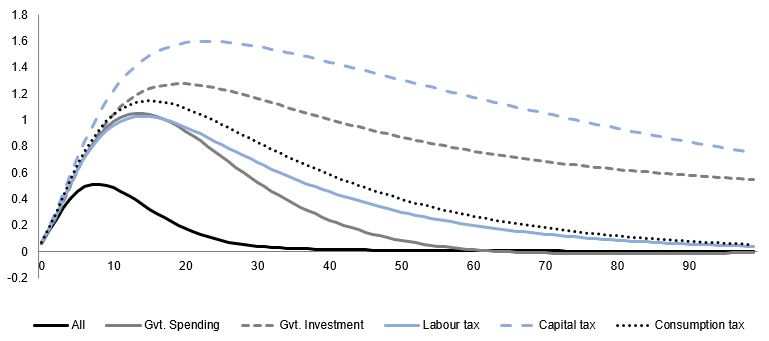
\includegraphics[width=15cm, trim =0 0 0 0]{Debt.jpg} \\ 
			\end{tabular}
			
		}
	\end{minipage}
	
	\subsection{The role of automatic stabilisers}
	
	Assumptions regarding the role of automatic stabilisers also play an important role in debt dynamics. In the baseline results discussed above, the coefficients measuring the contemporaneous response of fiscal variables to output were set at their estimated values (as shown in Table \ref{tab_prior_est} in the Appendix ). 

	Figure \ref{fig_stab_debt} presents government debt dynamics following a shock to government consumption spending and assuming all fiscal instruments adjust to stabilise debt. The figure shows results for four different assumptions regarding the automatic response of fiscal instruments to output fluctuations: no automatic response, estimated response, twice the estimated response, and three times the estimated response.
	
	Stronger automatic responses reduce short-run fluctuations, as reflected in the more muted short-term response of debt to the spending shock. However, stronger automatic responses could impose other long-run costs. Higher government spending raises output, which, under the estimated fiscal rules, indices an increase in capital and labour taxes and a decline in transfers. This, in turn, lowers output. This dynamic is more pronounced under stronger automatic stabilisers. The decline in output over the longer term reduces tax revenues, resulting a slightly more persistent deviation from steady state debt (see Figure \ref{fig_stab_debt}).   
	
	\begin{minipage}{\linewidth}
		
		\makebox[\linewidth]{
			\begin{tabular}{P{15cm}}
				\captionof{figure}{Role of automatic stabilisers in debt dynamics}\label{fig_stab_debt}
				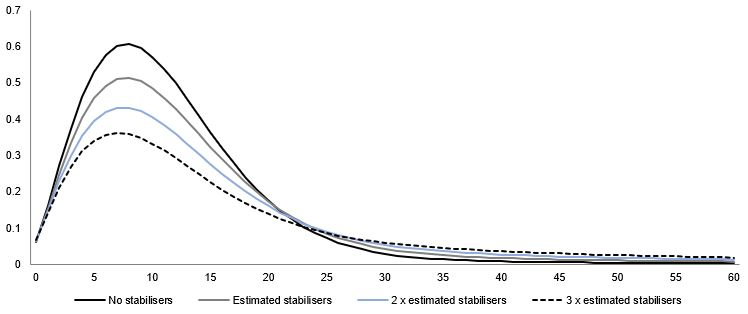
\includegraphics[width=15cm, trim =0 0 0 0]{Auto_stab.jpg} \\ 
			\end{tabular}
			
		}
	\end{minipage}
	
	
	
	\section{Conclusion} \label{con_dsge}
	
	In this paper, an open-economy fiscal DSGE model for the South African economy was constructed. The model includes a detailed fiscal block, as well as several other characteristics that make estimation feasible. 
	
	The estimated model fits the data reasonably well and was used to simulate the effect of innovations to the different fiscal instruments on macroeconomic aggregates, including GDP, private consumption and investment. The results highlight the fact that the fiscal policy process is highly complex and that the impact of fiscal policy decisions on macroeconomic aggregates depends crucially on assumptions about which fiscal instruments adjust to stabilise debt. 
	
	Policy simulations indicate that government spending and investment multipliers are generally positive, albeit smaller than one. Multipliers are also generally smaller than the estimates presented reduced-form modelling approaches, consistent with the idea that spending multipliers are smaller in open-economy settings. Secondly, the estimates indicate that taxes are highly distortionary, with large negative multipliers for private consumption and investment. In contrast, the impact of tax shocks on output is highly ambiguous, with assumptions regarding which instruments adjust to debt and the size of automatic stabilisers playing an important role. Finally, a look at debt dynamics indicates that government consumption spending and, to a slightly lesser extent, labour and consumption taxes are the most effective instruments for stabilising debt after a fiscal shock. This highlights an important finding: cuts in government consumption expenditure, combined with some measure of tax increases, present the most effective options when it comes to the need for fiscal consolidation. 
	
	That being said, conclusions about the effects of fiscal policy depend crucially on the nature of the underlying fiscal rules. As such, it is important for the researcher, and policy maker, to understand the different dynamics under different assumptions regarding the functional form of said rules.  
	
	This paper provides some insight into how fiscal policy decisions affect the economy. While the underlying dynamics are complex, the rules are relatively simple and the model economy could be expanded to include even more realistic assumptions. These could include distinguishing between productive and unproductive government spending, detailed modelling of monetary	policy behaviour, regime-switching fiscal policy, expanding the model to account for differing trends in fiscal variables, and introducing fiscal foresight in the open-economy setting.\footnote{\cite{jooste2017} incorporate an ad hoc measure of fiscal foresight in a calibrated, closed-economy DSGE model for South Africa.} Additionally, the analysis could be extended in order to consider optimal fiscal rules, as well as the differentiated impact of permanent versus temporary innovations to fiscal instruments. 
	
\newpage
\thispagestyle{plain}
\singlespacing
\nocite{}
\bibliographystyle{chicago}
\bibliography{bib}

\newpage
\appendix 

\setcounter{table}{0} \renewcommand{\thetable}{A.\arabic{table}}
\setcounter{section}{0}
\setcounter{subsection}{0}
\renewcommand{\thesection}{A.\arabic{section}}  

\setcounter{equation}{0}
\renewcommand\theequation{A.\arabic{equation}}	 

\section*{Appendix} \label{app}

\section{The log-linearised model} 
	

	\subsection{Fiscal and monetary authorities}
	
	Expressing the fiscal authority's budget constraint (\ref{fisc_budget}) as a share of nominal output results in the following expression for the budget constraint:
	
	\begin{multline} \label{fisc_share}
	s_{G,t}=\tau_t^c\frac{P_{C,t}C_t}{P_{Y,t}Y_t}+\tau_t^w\frac{W_{t}N_t}{P_{Y,t}Y_t}-\frac{P_{I_G,t}I_{G,t}}{P_{Y,t}Y_t}+\tau_t^ku_t\frac{R_{K,t}K_t}{P_{Y,t}Y_t}-\tau_t^k\left(\Gamma_u(u_t)+\delta\right)\frac{P_{I,t}K_t}{P_{Y,t}Y_t}\\
	+\frac{B_{t+1}}{R_tP_{Y,t}Y_t}-\frac{B_t}{P_{Y,t}Y_t} -s_{TR,t}
	\end{multline}
	
	where $s_{G,t}=P_{G,t}G_t/P_{Y,t}Y_t$ and $s_{TR,t}=TR_t/P_{Y,t}Y_t$ represents that shares of the public consumption good and transfer in nominal output.
	
	Applying the above-mentioned stationarity inducing transformation, the budget constraint (\ref{fisc_share}) can be expressed:
	
	\begin{multline}
	s_{G,t}=\tau_t^c\frac{p_{C,t}c_t}{p_{Y,t}y_t}+\tau_t^w\frac{w_{t}N_t}{p_{Y,t}y_t}-\frac{p_{I_G,t}i_{G,t}}{p_{y,t}y_t}+\tau_t^ku_t\frac{r_{K,t}k_tg_{z,t}^{-1}}{p_{Y,t}y_t}-\tau_t^k\left(\Gamma_u(u_t)+\delta\right)\frac{p_{I,t}k_tg_{z,t}^{-1}}{p_{Y,t}y_t}\\
	+\frac{b_{t+1}R_t^{-1}}{p_{Y,t}y_t}-\frac{b_t\pi_{C,t}^{-1}g_{z,t}^{-1}}{p_{Y,t}y_t}-s_{TR,t}
	\end{multline}
	
	where $b_{t+1}=B_{t+1}/z_tP_{C,t}$.
	
	The following log-linearised expression is obtained (recalling that $u=1$, $\Gamma_u(1)=0$ and $\Gamma_u^{'}(1)=r_Kp_I^{-1}$):
	
	\begin{align}
	\hat{s}_{G,t}=&\frac{p_C c}{p_Y y}\Big(\hat{\tau}_t^c+\tau^c\left(\hat{p}_{C,t}+\hat{c}_t-\hat{p}_{Y,t}-\hat{y}_t\right)\Big)\\
	&+\frac{wN}{p_Y y}\Big(\hat{\tau}_t^w+\tau^w\left(\hat{w}_{t}+\hat{N}_t-\hat{p}_{Y,t}-\hat{y}_t\right)\Big)\nonumber\\
	&-\frac{p_{I_G} i_G}{p_Y y}\Big(\hat{p}_{I_G,t}+\hat{i}_{G,t}-\hat{p}_{Y,t}-\hat{y}_t\Big)\nonumber\\
	&+\frac{r_Kkg_z^{-1}}{p_Y y}\Big(\hat{\tau}_t^k+\tau^k\left(\hat{u}_t+\hat{r}_{K,t}+\hat{k}_t-\hat{g}_{z,t}-\hat{p}_{Y,t}-\hat{y}_t\right)\Big)\nonumber\\
	&-\frac{p_Ikg_z^{-1}}{p_Y y}\Big(\gamma_{u,1}\hat{u}_t+\tau^k\delta\left(\hat{\tau}_t^k+\hat{p}_{I,t}+\hat{k}_t-\hat{g}_{z,t}-\hat{p}_{Y,t}-\hat{y}_t\right)\Big)\nonumber\\
	&+\frac{bR^{-1}}{p_Yy}\Big(\hat{b}_{t+1}-\hat{r}_t-\hat{p}_{Y,t}-\hat{y}_t\Big)-\frac{b\pi_C^{-1}g_z^{-1}}{p_Yy}\Big(\hat{b}_t-\hat{\pi}_{C,t}-\hat{g}_{z,t}-\hat{p}_{Y,t}-\hat{y}_t\Big)\nonumber\\
	&-\hat{s}_{TR,t}\nonumber
	\end{align} 
	
	where
	
	\begin{equation}
	\hat{s}_{G,t}=s_G\left(\hat{p}_{G,t}+\hat{g}_t-\hat{p}_{Y,t}-\hat{y}_t\right)
	\end{equation}
	
	
	Finally, the behaviour of the monetary authority is fully described by the simple log-linear Taylor rule presented in the main text (equation (\ref{mon_pol})).
	
	
	
	
	

\newpage
\begin{table}[h]
	\small
	\centering
	\captionsetup{skip=6pt}
	\caption{Present-value multipliers: Gvt. spending and investment respond}
	\begin{tabular}{p{2cm} P{1.25cm} P{1.25cm} P{1.25cm} P{1.25cm} P{1.25cm}} 
		\toprule
		Variable& Q1 & Q4 & Q8 & Q20 & $\infty$ \\
		\hline
		\multicolumn{6}{l}{\textbf{Government consumption multiplier}} \\
		\hline
		$\frac{\Delta Y}{\Delta G}$ &0.05&0.26&0.31&0.31&0.29\\
		$\frac{\Delta C}{\Delta G}$ &-0.80&-0.67&-0.56&-0.41&-0.39\\
		$\frac{\Delta I}{\Delta G}$ &-0.06&-0.08&-0.09&-0.10&-0.09\\
		\hline
		\multicolumn{6}{l}{\textbf{Government investment multiplier}} \\
		\hline
		$\frac{\Delta Y}{\Delta I_G}$ &0.59&0.67&0.64&0.59&0.58\\
		$\frac{\Delta C}{\Delta I_G}$ &-0.03&-0.03&-0.03&0.02&0.03\\
		$\frac{\Delta I}{\Delta I_G}$ &-0.05&-0.07&-0.08&-0.07&-0.06\\
		\hline
		\multicolumn{6}{l}{\textbf{Labour tax multiplier}} \\
		\hline
		$\frac{\Delta Y}{\Delta T^w}$ &-0.45&-0.39&-0.27&-0.11&-0.09\\
		$\frac{\Delta C}{\Delta T^w}$ &-0.63&-0.82&-1.02&-1.19&-1.19\\
		$\frac{\Delta I}{\Delta T^w}$ &-0.01&-0.05&-0.11&-0.17&-0.17\\
		\hline
		\multicolumn{6}{l}{\textbf{Capital tax multiplier}} \\
		\hline
		$\frac{\Delta Y}{\Delta T^k}$ &-0.19&-0.14&0.03&0.27&0.29\\
		$\frac{\Delta C}{\Delta T^k}$ &-0.04&-0.35&-0.71&-1.07&-1.08\\
		$\frac{\Delta I}{\Delta T^k}$ &-0.04&-0.14&-0.26&-0.38&-0.38\\
		\hline
		\multicolumn{6}{l}{\textbf{Consumption tax multiplier}} \\
		\hline
		$\frac{\Delta Y}{\Delta T^c}$ &-0.23&-0.22&-0.09&0.10&0.12\\
		$\frac{\Delta C}{\Delta T^c}$ &-0.20&-0.58&-0.91&-1.17&-1.17\\
		$\frac{\Delta I}{\Delta T^c}$ &-0.01&-0.07&-0.14&-0.23&-0.23\\
		\toprule
	\end{tabular}
	\label{pv_spend_tools}
\end{table}

\newpage
\begin{table}[h!]
	\small
	\centering
	\captionsetup{skip=6pt}
	\caption{Present-value multipliers: Taxes respond}
	\begin{tabular}{p{2cm} P{1.25cm} P{1.25cm} P{1.25cm} P{1.25cm} P{1.25cm}} 
		\toprule
		Variable& Q1 & Q4 & Q8 & Q20 & $\infty$ \\
		\hline
		\multicolumn{6}{l}{\textbf{Government consumption multiplier}} \\
		\hline
		$\frac{\Delta Y}{\Delta G}$ &-0.23&0.08&0.14&0.17&0.16\\
		$\frac{\Delta C}{\Delta G}$ &-0.87&-0.76&-0.70&-0.63&-0.62\\
		$\frac{\Delta I}{\Delta G}$ &-0.09&-0.12&-0.14&-0.17&-0.16\\
		\hline
		\multicolumn{6}{l}{\textbf{Government investment multiplier}} \\
		\hline
		$\frac{\Delta Y}{\Delta I_G}$ &0.48&0.56&0.52&0.48&0.48\\
		$\frac{\Delta C}{\Delta I_G}$ &-0.06&-0.11&-0.17&-0.23&-0.23\\
		$\frac{\Delta I}{\Delta I_G}$ &-0.06&-0.09&-0.12&-0.14&-0.13\\
		\hline
		\multicolumn{6}{l}{\textbf{Labour tax multiplier}} \\
		\hline
		$\frac{\Delta Y}{\Delta T^w}$ &-0.35&-0.33&-0.32&-0.30&-0.30\\
		$\frac{\Delta C}{\Delta T^w}$ &-0.60&-0.58&-0.56&-0.54&-0.53\\
		$\frac{\Delta I}{\Delta T^w}$ &0.01&0.03&0.05&0.07&0.07\\
		\hline
		\multicolumn{6}{l}{\textbf{Capital tax multiplier}} \\
		\hline
		$\frac{\Delta Y}{\Delta T^k}$ &-0.04&0.05&0.13&0.20&0.21\\
		$\frac{\Delta C}{\Delta T^k}$ &-0.02&0.20&0.38&0.53&0.53\\
		$\frac{\Delta I}{\Delta T^k}$ &-0.02&-0.05&-0.08&-0.12&-0.13\\
		\hline
		\multicolumn{6}{l}{\textbf{Consumption tax multiplier}} \\
		\hline
		$\frac{\Delta Y}{\Delta T^c}$ &-0.10&-0.10&-0.08&-0.06&-0.05\\
		$\frac{\Delta C}{\Delta T^c}$ &-0.17&-0.19&-0.18&-0.16&-0.15\\
		$\frac{\Delta I}{\Delta T^c}$ &0.01&0.03&0.05&0.07&0.07\\
		\toprule
	\end{tabular}
	\label{pv_tax_tools}
\end{table}

	
\end{document}
